\section{Status Register}
Uno dei registri interni al processore è lo \emph{Status Register}, si compone di 8 bit ognuno dei quali ha un significato e descrive una caratteristica dello stato interno del processore.

\begin{figure}[H]
    \centering
    
\includegraphics[width=250px]{images/4_Status_register/status_register.png}
\end{figure}

Questo registro può essere letto per intero leggendo l'ultimo indirizzo dello spazio delle periferiche.

\subsection{Carry bit}
Il bit meno significativo dello status register è detto \emph{carry bit} o \emph{carry flag} ed indica se c'è stato un riporto durante una somma o un presito durante una sottrazione.

La ALU prende quasi sempre due parametri (solo uno quando fa una negazione dei bit o cambia di segno) e restituisce un solo risultato, le operazioni con la ALU inoltre sono distruttive in quanto scrivono il risultato all'interno del registro usato come destinazione:

\begin{verbatim}
    ADD r7, r9  #  r7 <- r7 + r9
\end{verbatim}

La ALU fornisce un risultato a 8 bit, tuttavia è in grado di prendere il nono bit in uscita dalla somma richiesta e di aggiornare il carry flag, quindi il CF diventa 1 se la somma non è rappresentabile su 8 bit.

Anche nella sottrazione questo flag viene aggiornato, in particolare nella differenza A-B se A è minore di B allora il carry flag indica che c'è stato un prestito. Nella pratica quello che viene eseguito dalla ALU è:
$$ 12 - 17 = (256 + 12) - 17 = 251 $$
251 è il valore -5 espresso in complemento a 2.

Oltre che per il riporto o il prestito il CF può essere utilizzato per eseguire operazioni su più byte: 1000 non è rappresentabile su un singolo byte, possiamo pertanto suddividerlo in una parte alta ed in una parte bassa:
$$ 1000 - 248  = \text{0x03E8} - \text{0x00F8} $$

\begin{verbatim}
    MOV r1, 0x03 # r1 <- 0x03
    MOV r0, 0xE8 # r0 <- 0xE8
    # indico con r1:r0
    
    MOV r3, 0x00 # r3 <- 0x00
    MOV r2, 0xF8 # r2 <- 0xF8
    # indico con r3:r2
    
    SUB r0, r2   # r0 <- r0 - r2
    SBC r1, r3   # r1 <- r1 - r3 - CF
\end{verbatim}
usando l'istruzione SBC - \emph{subtract with carry} abbiamo scomposto una operazione su 16 bit in operazioni su 8 bit, questo possiamo scalarlo anche per operazioni a 32 bit e così via.

Per eseguire la stessa cosa con una somma esiste l'istruzione ADC - \emph{add with carry}.

\subsection{Zero bit}
Il secondo bit indica se l'ultima operazione aritmetica ha generato un risultato composto da tutti 0.
\begin{verbatim}
    MOV r7, 11
    MOV r8, 11
    SUB r7, r8 # il risultato è zero quindi Z = 1
\end{verbatim}

Possiamo usarlo per eseguire test di uguaglianza, se facendo una sottrazione lo zero flag va ad 1 allora i numeri erano uguali. La sottrazione tuttavia è distruttiva, per fare le comparazioni quindi esiste un'altra istruzione: CP, fa una sottrazione, aggiorna i flag dello SREG ma butta via il risultato anziché sovrascrivere il registro.
\begin{verbatim}
    CP r7, r8
\end{verbatim}

Un altro utilizzo lo si ha nel controllare se un bit ha un determinato valore, i microcontrollori hanno delle periferiche per leggere valori digitali dall'esterno, supponiamo pertanto di avere questo circuito:

\begin{figure}[H]
    \centering
    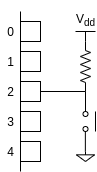
\includegraphics{images/4_Status_register/example_and_1.png}
\end{figure}
e di aver letto il valore dei pin nel registro r7 (vedremo come si fa più avanti). Il terzo bit di questo registro ora ha il valore del pin, vogliamo pertanto isolare quel singolo bit e sapere che valore ha: applichiamo una maschera eseguendo l'AND logico:
\begin{figure}[H]
    \centering
    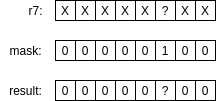
\includegraphics[width=150px]{images/4_Status_register/example_and_2.png}
\end{figure}

\begin{verbatim}
    # in r7 abbiamo il valore dei pin
    MOV r9, 0x04
    AND r9, r7
\end{verbatim}
ho quindi isolato il bit 2 ed inoltre ha aggiornato i flag, controllando lo Z flag posso trovarvi 1: ho quindi prodotto uno zero ed il pulsante era chiuso, oppure potrei trovarvi 0: in tal caso il pin era ad 1 e quindi il pulsante era aperto.

\subsection{Half carry bit}
Il bit H dello SREG indica se nell'ultima operazione aritmetica si è generato un half carry. Un half carry è un riporto che va dal terzo bit al quarto bit:

\begin{figure}[H]
    \centering
    
\includegraphics[width=150px]{images/4_Status_register/half_carry.png}
\end{figure}
questo flag è utile solo nelle operazioni con codifica BCD.

\subsubsection{Binary Coded Digit}
La codifica BCD prevede l'uso di 4 bit per rappresentare le cifre decimali, si usando i numeri da 0 a 9 esattamente come fossero rappresentati in binario. Supponiamo di dover sommare due numeri a due cifre in questa codifica, possiamo distinguere 3 casi:
\begin{itemize}
    \item 15 + 13 = 28
    
    La somma con la ALU è corretta anche leggendola in BCD
    
    \item 15 + 16 = 2B
    
    La somma con la ALU non è corretta in quanto abbiamo che la seconda cifra non ha fatto il riporto verso la prima, possiamo accorgercene controllando le singole cifre e vedendo che è maggiore di 9. Possiamo aggiustarla semplicemente sommando 6 (tolgo 10 per prendere ciò che c'è in più e sommo 16 per il riporto).
    
    2B + 6 = 31

    \item 18 + 19 = 31
    
    La somma non è corretta ma sembra esserlo perché le cifre sono tutte rappresentabili in BCD.
    Non abbiamo modo di accorgerci dell'errore.
    Questo errore è correlato al riporto tra i primi quattro bit ed i secondi quattro, intercettando questo riporto possiamo accorgerci dell'errore e fixarlo.
    Per fixare anche qui mi basta aggiungere 6 in quanto è ciò che ha portato in più nella seconda cifra per fare il riporto.
\end{itemize}

\subsection{Bit S V N}
Se eseguo una somma interpretando i numeri come numeri con segno, quindi in complemento a 2, il carry bit non è affidabile:
$$ 100 + 100 = 0x64 + 0x64 = 0xC8 $$
questa somma non ha emesso carry ed il bit più significativo è 1 quindi ci segna che il numero è negativo ma non dovrebbe esserlo in quanto entrambi gli addendi sono positivi.

In questo caso non possiamo affidarci al carry flag per sapere se la nostra somma è andata a buon fine. Per queste situazioni esistono altri 3 flag:
\begin{itemize}
    \item N \emph{negative flag}: copia del bit più significativo prodotto dall'operazione aritmetica
    \item V \emph{overflow flag}: è il valore prodotto da $N \oplus C$ ed indica e il risultato è corretto leggendolo come complemento a 2.
    \item S \emph{sign flag}: ci dice quale sarebbe stato il segno se il risultato fosse stato coretto
\end{itemize}

\subsection{Bit T}
Questo bit non ha un significato specifico, può essere settato e resettato dall'utente utilizzando due istruzioni. Sta per \emph{temporary flag}.

\subsection{Interrupt bit}
Questo flag è settabile e resettabile dal programmatore, serve ad abilitare o disabilitare la logica di interruzione.
Di norma è a 0.

